\section{Why the Development Gate Failed}
\label{sec:analysis}

\subsection{Observed development frontier}

Figure~\ref{fig:pareto} plots the five observed development systems. It is descriptive: it contains no untouched examples, confidence intervals, or post-gate threshold search. The dashed frontier connects Direct and CoT/PoT; Static Nexus, ReAct, and Selective Nexus lie below that observed development frontier.

\begin{figure}[t]
  \centering
  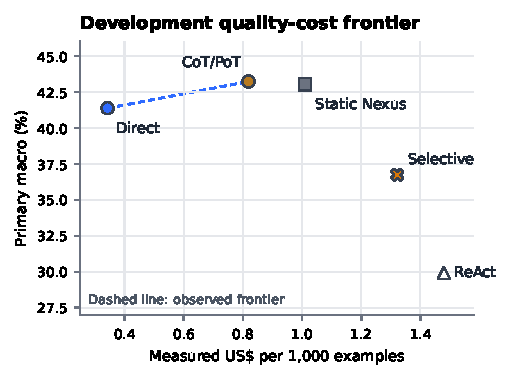
\includegraphics[width=\columnwidth]{figures/development_quality_cost.pdf}
  \Description{Development-only scatter plot of primary macro quality against measured US dollars per one thousand examples. Direct and CoT/PoT form the dashed observed frontier. Static Nexus, Selective Nexus, and ReAct lie below it.}
  \caption{Development-only quality--cost observations. These points triggered the preregistered stop and are not confirmatory results.}
  \label{fig:pareto}
\end{figure}

\subsection{Router gate}

Router labels were available for 200 examples across FinanceBench, FinQA, TAT-QA, and ConvFinQA. FinDER was excluded because no human-validated objective label was available. Only 10 examples were ReAct-correct and Static-Nexus-incorrect. At least one cross-validation fold therefore had fewer than five usable benefit examples, activating the preregistered rule fallback rather than the logistic model.

\begin{table}[t]
  \caption{Development-only router gate. Accuracy and cost use the 200-example objective router set, not the three-task primary macro in Table~\ref{tab:development-gate}.}
  \label{tab:router-gate}
  \centering
  \small
  \begin{tabular}{lr}
    \toprule
    Gate quantity & Outcome \\
    \midrule
    Objective-labeled examples & 200 \\
    ReAct-only benefit labels & 10 \\
    Selected policy & Rule fallback \\
    Lexical-coverage threshold & 0.666667 \\
    Retrieval-margin threshold & 1.0 \\
    Escalation rate & 70\% \\
    Offline branch estimate & 0.280 \\
    Observed selective exact accuracy & 0.295 \\
    Static exact accuracy & 0.395 \\
    Observed selective mean cost & US\$0.001431 \\
    \bottomrule
  \end{tabular}
\end{table}

The offline saved-branch simulation estimated 0.280 accuracy; the fresh deployable selective rerun achieved 0.295, still 0.100 below always static on the router set. Across the four objectively labeled datasets, there were only 10 ReAct-only successes versus 42 Static-only successes. This imbalance explains why a broad escalation rule could not recover the rare benefit cases without routing many cases to the weaker iterative path. It does not identify a causal failure taxonomy; that analysis was not opened on the final set.

\subsection{Implication for a later study}

A credible redesign needs a new development pool and a routing target that can be estimated despite rare ReAct-only events---for example, richer uncertainty signals, calibrated post-static validation whose full cost is counted, or a different iterative expert that first demonstrates complementary accuracy. Any redesign must pass a newly frozen gate before the existing 900-example manifest is opened. Reusing the present development outcomes to tune and then treating them as evaluation would invalidate the protocol.
